\input{pack.tex}

\title{\LARGE \textbf{MiniRT} - Notes}
\author{\large Lucie Le Briquer}
\date{\today}

\begin{document}
\maketitle
\tableofcontents
\newpage\section{Génération des rayons}
\begin{center}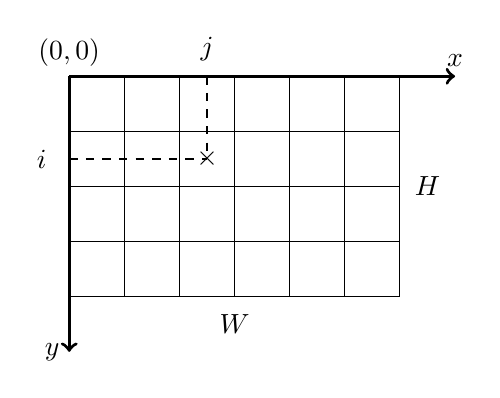
\begin{tikzpicture}[scale=0.7]
	\draw[step=1.0,black,thin] (0,0) grid (6,4);
	\draw[->,very thick] (0,4)--(7,4);
	\draw (7,4) node[above]{$x$};
	\draw[->,very thick] (0,4)--(0,-1);
	\draw (0,-1) node[left]{$y$};
	\draw (0,4) node[left,above]{$(0,0)$};
	\draw (2.5,2.5) node{$\times$};
	\draw (3,-0.5) node{$W$};
	\draw (6.5,2) node{$H$};
	\draw (-0.5,2.5) node{$i$};
	\draw (2.5,4.5) node{$j$};
	\draw[dashed] (0,2.5)--(2.5,2.5);
	\draw[dashed] (2.5,4)--(2.5,2.5);
\end{tikzpicture}
\hspace{1cm}
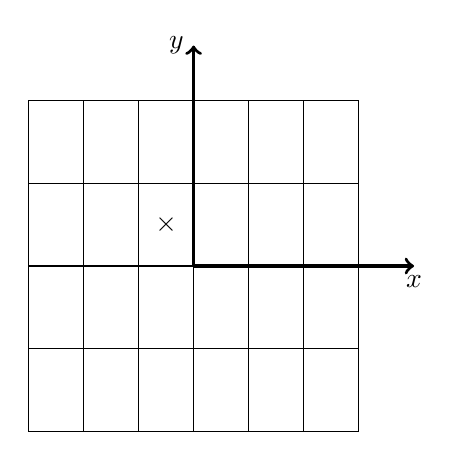
\begin{tikzpicture}[scale=0.7]
	\draw[step=1,yscale=1.5,black,thin] (0,0) grid (6,4);
	\draw[->,very thick] (3,3)--(7,3);
	\draw (7,3) node[below]{$x$};
	\draw[->,very thick] (3,3)--(3,7);
	\draw (3,7) node[left]{$y$};
	\draw (2.5,3.75) node{$\times$};
\end{tikzpicture}\end{center}
\dd\ni On cherche a remplir l'image pixel par pixel, on a $i$ correspondant a la
ligne du pixel et $j$ a sa colonne. On va d'abord normaliser les coordonnees
selon la largeur et la hauteur de l'ecran pour travailler avec une image carree.
On note :
$$\text{pixNorm}_x=\frac{j + 0.5} W \etsp\text{pixNorm}_y\frac{i + 0.5} H$$
\ni On effectue ensuite une translation pour centrer le repere sur le milieu de
l'ecran ainsi qu'une inversion de l'axe $y$. Ainsi :
$$\text{pixScreen}_x=2 \times\text{pixNorm}_x -1 \etsp \text{pixScreen}_y = 1 -
2\times \text{pixNorm}_y$$
\ni Il reste ensuite a prendre en compte la FOV donnee en parametre :
$$\text{pixFinal}_x = \text{pixScreen}_x \times \text{ratio}
\times\tan\left(\frac{\text{FOV}} 2\right)\etsp \text{pixFinal}_y = 
\text{pixScreen}_y \times\tan\left(\frac{\text{FOV}} 2\right)$$
\ni Finalement :
$$\text{pixFinal}_x = \left(2\times \frac{j+0.5}{W}- 1\right)
\times \text{ratio}\times\tan\left(\frac{\text{FOV}} 2\right)$$
$$\text{pixFinal}_y = \left(1 - 2\times \frac{i+0.5}{H}\right)
\times\tan\left(\frac{\text{FOV}} 2\right)$$


\newpage\section{Rotation de la caméra}



\newpage\section{Interaction rayon-sphère}
\ni Soit $(o_r, \vec{d}_r)$ le rayon lance pour lequel on cherche une intersection
avec une sphere ($o_r$ est l'origine du rayon, $\vec{d}_r$ sa direction). Soit $o$ le
centre de la sphere $\Sl$ et $r$ son rayon. On cherche donc un point $p$ de la forme
:
$$p = o_r + \bt \vec{d}_r\quad \bt>0$$
\ni intersectant la sphere, donc verifiant :
$$\|p - o\|^2 = r$$
\ni On veut donc :
\begin{align*}
	&\|o_r - o + \bt \vec{d}_r\|^2=r^2\\
	\Lra\quad&\bt^2\|\vec{d}_r\|^2 + 2\bt\scl{\vec{d}_r, o_r - o} 
	+\|o_r - o\|^2 =r^2\\
	\Lra\quad&\bt^2 + 2\bt\scl{\vec{d}_r, o_r - o} +\|o_r - o\|^2 =r^2
\end{align*}
\ni Le determinant est :
$$\Delta = 4\times\left(\scl{\vec{d}_r, o - o_r}^2 - \|o - o_r\|^2 - 
r^2\right)$$
\ni Il ne reste plus qu'a determiner la plus petite racine positive si elle
existe. Si le determinant est negatif ou que les racines (ou la racine double)
sont negatives, l'intersection n'est pas visible depuis la camera.

\section{Interaction rayon-plan}
\ni Soit $(o,\vec{n})$ le plan $\Pl$, ou $\vec{n}$ est la normale au plan et $o$
un point du plan. Comme precedemment on cherche un point $p$ de la forme :
$$p = o_r + \bt \vec{d}_r\quad \bt>0$$
\ni intersectant le plan, donc verifiant :
$$\scl{p - o, \vec{n}} = 0$$
\ni On veut donc :
\begin{align*}
	&\scl{o_r + \bt \vec{d}_r - o + \bt, \vec{n}}=0\\
	\Lra\quad&\scl{o_r - o, \vec{n}} + \bt \scl{\vec{d}_r,\vec{n}}=0\\
\end{align*}
Ainsi :
$$\bt = \frac{\scl{o - o_r, \vec{n}}}{\scl{\vec{d}_r,\vec{n}}}$$
\ni Si $\bt$ est bien positif il y a une intersection visible avec le plan.

\newpage\section{Interaction rayon-triangle}
\ni Soit $(a,b,c)$ les sommets du triangle $T$. Une premiere etape et de
verifier qu'il existe un $\bt$ tel que $p$ soit dans le plan du triangle, on a
donc besoin d'une normale au triangle, on prend par exemple $\vec{n} = (b - a) \wedge(c - a)$
\begin{center}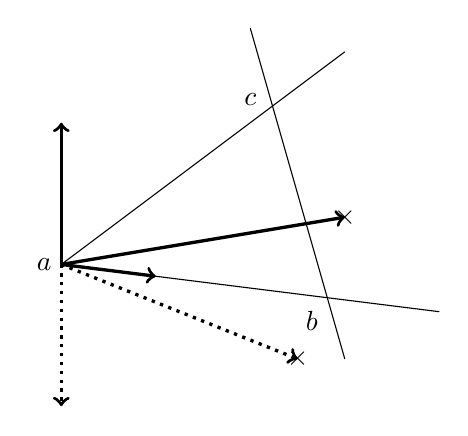
\begin{tikzpicture}[scale=0.6]
	\draw (0,0)--(8,-1);
	\draw (0,0)--(6,4.5);
	\draw[->,very thick] (0,0)--(2,-0.25);
	\draw (0,0) node[left]{$a$};
	\draw (5.3,-1.2) node{$b$};
	\draw (4,3.5) node{$c$};
	\draw (4,5)--(6,-2);
	\draw[->,very thick] (0,0)--(0,3);
	\draw[->,dotted,very thick] (0,0)--(0,-3);
	\draw (6,1) node{$\times$};
	\draw[->,very thick] (0,0)--(6,1);
	\draw (5,-2) node{$\times$};
	\draw[->,very thick,dotted] (0,0)--(5,-2);
\end{tikzpicture}\end{center}

\newpage\section{Interaction rayon-carré}

\newpage\section{Interaction rayon-cylindre}
\ni Soit $(o,X,Y,Z)$ le repère du cylindre $\Cl$. Le point $p\in\Cl$ ssi
$$x_p^2 + y_p^2 = r^2\etsp|z_p|\leq\frac h 2$$
\ni avec $(x_p,y_p,z_p)$ les coordonnées de $p$ dans le repère du
cylindre. Pour déterminer les vecteurs $(X,Y,Z)$ il suffit d'utiliser la même
construction de base vue précédemment avec comme axe de départ l'axe du cylindre.
\img{0.2}{cylindre}
\dd Le point $p$ est de la forme $o_R + \bt d_R$ où $o_R$ est l'origine du rayon et
$d_R$ sa direction. Ainsi :
$$x_p = \lng p - o, X\rng = \bt\scl{d_R, X} + \scl{o_r - o, X}$$
$$y_p = \lng p - o, Y\rng = \bt\scl{d_R, Y} + \scl{o_r - o, Y}$$
Donc,
\begin{align*}
	x_p^2 + y_p^2 = &\left(\scl{d_R,X}^2 + \scl{d_r,Y}^2\right) \bt^2\\
		&+2\left(\scl{d_R,X}\scl{o_R-o,X}+\scl{d_R,Y}\scl{o_R-o,Y}\right) \bt \\
		&+\left(\scl{o_R-o, X}^2 + \scl{o_R-o,Y}^2\right)
\end{align*}
\ni$\bt$ vérifie donc une équation du second degré $a\bt^2+b\bt+c=0$ avec :
$$\sys{a = \scl{d_R,X}^2 + \scl{d_r,Y}^2\\\\
b = 2\left(\scl{d_R,X}\scl{o_R-o,X}+\scl{d_R,Y}\scl{o_R-o,Y}\right) \\\\
c = \scl{o_R-o, X}^2 + \scl{o_R-o,Y}^2 - r^2
}$$
\ni Il ne reste plus qu'à vérifier que pour un des deux $\bt$ on obtient
un point $p$ vérifiant $|z_p|\leq\frac h 2$ sachant que :
$$z_p = \lng p - o, Z\rng = \bt\scl{d_R, Z} + \scl{o_r - o, Z}$$

\end{document}
